\documentclass[dvipdfmx]{jsarticle}


\usepackage{tcolorbox}
\usepackage{color}
\usepackage{listings, plistings}

%% ノート/latexメモ
%% http://pepper.is.sci.toho-u.ac.jp/pepper/index.php?%A5%CE%A1%BC%A5%C8%2Flatex%A5%E1%A5%E2

%% JavaScriptの設定
%% https://e8l.hatenablog.com/entry/2015/11/29/232800
\lstdefinelanguage{javascript}{
  morekeywords = [1]{ %keywords
    await, break, case, catch, class, const, continue, debugger, default, delete, 
    do, else, enum, export, extends, finally, for, function, function*, if, implements, import, in, 
    instanceof, interface, let, new, package, private, protected, public, return, static, super,
    switch, this, throw, try, typeof, var, void, while, with, yield, yield*
  },
  morekeywords = [2]{ %literal
    false, Infinity, NaN, null, true, undefined
  },
  morekeywords = [3] { %Classes
    Array, ArrayBuffer, Boolean, DataView, Date, Error, EvalError, Float32Array, Float64Array,
    Function, Generator, GeneratorFunction, Int16Array, Int32Array, Int8Array, InternalError,
    JSON, Map, Math, Number, Object, Promise, Proxy, RangeError, ReferenceError, Reflect,
    RegExp, Set, String, Symbol, SyntaxError, TypeError, URIError, Uint16Array, Uint32Array,
    Uint8Array, Uint8ClampedArray, WeakMap, WeakSet
  },
  morecomment = [l]{//},
  morecomment = [s]{/*}{*/},
  morestring = [b]{"},
  morestring = [b]{'},
  alsodigit = {-},
  sensitive = true
}

%% 修正時刻: Tue 2022/03/15 10:04:41


% Java
\lstset{% 
  frame=single,
  backgroundcolor={\color[gray]{.9}},
  stringstyle={\ttfamily \color[rgb]{0,0,1}},
  commentstyle={\itshape \color[cmyk]{1,0,1,0}},
  identifierstyle={\ttfamily}, 
  keywordstyle={\ttfamily \color[cmyk]{0,1,0,0}},
  basicstyle={\ttfamily},
  breaklines=true,
  xleftmargin=0zw,
  xrightmargin=0zw,
  framerule=.2pt,
  columns=[l]{fullflexible},
  numbers=left,
  stepnumber=1,
  numberstyle={\scriptsize},
  numbersep=1em,
  language={Java},
  lineskip=-0.5zw,
  morecomment={[s][{\color[cmyk]{1,0,0,0}}]{/**}{*/}},
  keepspaces=true,         % 空白の連続をそのままで
  showstringspaces=false,  % 空白字をOFF
}
%\usepackage[dvipdfmx]{graphicx}
\usepackage{url}
\usepackage[dvipdfmx]{hyperref}
\usepackage{amsmath, amssymb}
\usepackage{itembkbx}
\usepackage{eclbkbox}	% required for `\breakbox' (yatex added)
\usepackage{enumerate}
\usepackage[default]{cantarell}
\usepackage[T1]{fontenc}
\fboxrule=0.5pt
\parindent=1em
\definecolor{mygrey}{rgb}{0.97, 0.97, 0.97}

\makeatletter
\def\verbatim@font{\normalfont
\let\do\do@noligs
\verbatim@nolig@list}
\makeatother

\begin{document}

%\anaumeと入力すると穴埋め解答欄が作れるようにしてる。\anaumesmallで小さめの穴埋めになる。
\newcounter{mycounter} % カウンターを作る
\setcounter{mycounter}{0} % カウンターを初期化
\newcommand{\anaume}[1][]{\refstepcounter{mycounter}{#1}{\boxed{\phantom{aa}\textnormal{\themycounter}\phantom{aa}}}} %穴埋め問題の空欄作ってる。
\newcommand{\anaumesmall}[1][]{\refstepcounter{mycounter}{#1}{\boxed{\tiny{\phantom{a}\themycounter \phantom{a}}}}}%小さい版作ってる。色々改造できる。

%% 修正時刻: Tue 2022/03/15 10:04:411


\section{テーブル(表)を作成する}

\subsection{作成する表のイメージ}

以下のような表を作成することとする。

\begin{table}[h]
 \caption{emp}
 \begin{center}
  \begin{tabular}[h]{|c|l|c|c|c|}
   \hline
   ID & 名前       & 年齢 & 誕生年 & 部署ID \\ \hline\hline
   1  & 菅原文太   & 40   & 1933   & 001    \\ \hline
   2  & 千葉真一   & 34   & 1939   & 002    \\ \hline
   3  & 北大路欣也 & 30   & 1943   & 003    \\ \hline
   4  & 梶芽衣子   & 26   & 1947   & 002    \\ \hline
  \end{tabular}
 \end{center}
\end{table}

\begin{table}[h]
 \caption{dep}
 \begin{center}
  \begin{tabular}{|l|c|} \hline
   ID   & 部署名 \\ \hline\hline
   001  & 総務部 \\ \hline
   002  & 営業部 \\ \hline
   003  & 経理部 \\ \hline
   004  & 開発部 \\ \hline
  \end{tabular}
 \end{center}
\end{table}

そして、上の2つの表から、以下の結合表を表示することとする。

\begin{table}[h]
 \begin{center}
  \begin{tabular}[h]{|c|l|c|c|c|}
   \hline
   ID & 名前       & 年齢  & 部署名 \\ \hline\hline
   1  & 菅原文太   & 40    & 総務部    \\ \hline
   2  & 千葉真一   & 34    & 営業部    \\ \hline
   3  & 北大路欣也 & 30    & 経理部    \\ \hline
   4  & 梶芽衣子   & 26    & 営業部    \\ \hline
  \end{tabular}
 \end{center}
\end{table}
 
\newpage
 
\subsection{テーブルの定義}

テーブルの定義を決める。

\begin{table}[ht]
 \caption{empテーブルの定義}
 \begin{center}
  \begin{tabular}{|l|l|l|} \hline
   項目 & 型 & オプション \\ \hline
   id   & int & primary key auto\_increment \\ 
   name & varchar(20) & not null \\ 
   age  & int & not null \\ 
   birthday & year & not null \\ 
   dept\_id & char(3) & \\ \hline
  \end{tabular}
 \end{center}
\end{table}

\textgt{型}

\begin{tabular}{ll}
 int型 & 整数。これがよく使われる。 \\
 varchar型 & 可変長の文字列型。ここでは最大20文字としている。(全角文字を使った場合) \\
 year型 & 年のみを扱う型。誕生の年だけを入力する。 \\
 char型 & 固定長の文字型。ここで半角で3文字としている。
\end{tabular}

\vspace{3mm}
\textgt{オプション}

\begin{tabular}{ll}
 primary key & 項目 id をデータの識別に使う。重複する値がないことが保証される。 \\
 auto\_increment & 自動連番。自動的に順に番号を振ってくれる機能を使う。 \\
 not null & 入力が必須。もしも入力しなかったら エラー になる。 \\
\end{tabular}

\vspace{3mm}
最後の dept\_id を not null にしなかったのは、部署ID のない社員もいるかもしれないからである。

\vspace{3mm}
deptテーブルは、このような定義になる。
 
\begin{table}[h]
 \caption{deptテーブルの定義}
 \begin{center}
  \begin{tabular}{|l|l|l|} \hline
   項目 & 型 & オプション \\ \hline
   id   & char(3) & primary key \\ 
   name & varchar(20) & not null \\ \hline
  \end{tabular}
 \end{center}
\end{table}

今回の場合、empテーブルには dept\_id が入っている。これは、deptテーブルの id のことである。
このことにより、empテーブルとdeptテーブルを結合させることができる。

このときの empテーブルの dept\_id のことを ``\textgt{外部キー}'' という。


\subsection{テーブルの作成}

テーブルを作成する前に、データベースの使用を宣言する。

\begin{tcolorbox}
 MariaDB [(none)]$>$ use sample; 
\end{tcolorbox}

以下のコマンドにより empテーブルを作成できる。

\begin{tcolorbox}
 MariaDB [sample]$>$ create table emp ( \\
 \hspace{6mm} \verb!->! id int primary key auto\_increment, (カンマ) \\
 \hspace{6mm} \verb!->! name varchar(20) not null, \\
 \hspace{6mm} \verb!->! age int not null, \\
 \hspace{6mm} \verb!->! birthday year not null, \\
 \hspace{6mm} \verb!->! dept\_id char(3) (カンマなし) \\
 \hspace{6mm} \verb!->! );
\end{tcolorbox}

同様に deptテーブルも作成する。

\begin{tcolorbox}
 MariaDB [sample]$>$ create table dept ( \\
 \hspace{6mm} \verb!->! id char(3) primary key, (カンマ) \\
 \hspace{6mm} \verb!->! name varchar(20) not null (カンマなし) \\
 \hspace{6mm} \verb!->! );
\end{tcolorbox}

\vspace{3mm}
\noindent ※
\quad 作成したテーブルの構造は以下のコマンドで確認できる。 \\
MariaDB [sample]$>$ \textsf{desc emp;}
\begin{verbatim}
+----------+-------------+------+-----+---------+----------------+
| Field    | Type        | Null | Key | Default | Extra          |
+----------+-------------+------+-----+---------+----------------+
| id       | int(11)     | NO   | PRI | NULL    | auto_increment |
| name     | varchar(20) | NO   |     | NULL    |                |
| age      | int(11)     | NO   |     | NULL    |                |
| birthday | year(4)     | NO   |     | NULL    |                |
| dept_id  | char(3)     | YES  |     | NULL    |                |
+----------+-------------+------+-----+---------+----------------+
\end{verbatim}

また、テーブルを作成したときのコマンドは以下で確認できる。\\
MariaDB [sample]$>$ \textsf{show create table emp;}
\begin{verbatim}
...(省略)... 
CREATE TABLE `emp` ( 
  `id` int(11) NOT NULL AUTO\_INCREMENT,
  `name` varchar(20) NOT NULL,
  `age` int(11) NOT NULL,
  `birthday` year(4) NOT NULL,
  `dept\_id` char(3) DEFAULT NULL,
  PRIMARY KEY (`id`)
) ENGINE=InnoDB DEFAULT CHARSET=utf8mb4
\end{verbatim}

\subsection{データの登録}

データの登録は、以下のコマンドでできる。

\begin{tcolorbox}
 MariaDB [sample]$>$ \textsf{insert into emp (name, age, birthday, dept\_id) values ('菅原文太', 40, 1933, '001');}
\end{tcolorbox}
\rightline{※ 各データの区切りは \textsf{,}(カンマ)}
\noindent
''id'' は auto\_increment なので、指定しない。\\
また、dept\_id は char(3) なので、\textsf{'001'} シングルクォーテーションを使って入力する。

画面の関係で一行で入力しづらければ、次のように二行で入力することもできる。

\begin{tcolorbox}
 MariaDB [sample]$>$ \textsf{insert into emp (name, age, birthday, dept\_id)} \\
 \hspace{6mm} \verb!->! \textsf{values ('千葉真一', 34, 1939, '002');}
\end{tcolorbox}

TeraPad などのエディタで記述しておいて、コピー\&貼り付け ですることもできる。

以下のようにすると、一度で入力できてしまう。

\begin{tcolorbox}
 MariaDB [sample]$>$ \textsf{insert into emp (name, age, birthday, dept\_id) values} \\
 \hspace{6mm} \verb!->! \textsf{('北大路欣也', 30, 1943, '003'),}   (カンマ) \\
 \hspace{6mm} \verb!->! \textsf{('梶芽衣子', 26, 1947, '002');}
\end{tcolorbox}

これも、エディタに記述しておいて、コピー\&貼り付けでも できる。

データの確認は次のコマンドでできる。

\begin{tcolorbox}
 MariaDB [sample]$>$ \textsf{select * from emp;}
\end{tcolorbox}

\begin{verbatim}
+----+------------+-----+----------+---------+
| id | name       | age | birthday | dept_id |
+----+------------+-----+----------+---------+
|  1 | 菅原文太   |  40 |     1933 | 001     |
|  2 | 千葉真一   |  34 |     1939 | 002     |
|  3 | 北大路欣也 |  30 |     1943 | 003     |
|  4 | 梶芽衣子   |  26 |     1947 | 002     |
+----+------------+-----+----------+---------+
\end{verbatim}

\subsection{ファイル読込みによるデータの登録}

同様に、deptテーブルについてもデータを登録する。

ただ、今度は 登録のための SQL文を外部ファイルに記述しておいて、
それを読み込むという方法で登録してみる。

\subsubsection{作業のためのフォルダを用意して、そこでファイルをつくる。}

ファイルを置くためのフォルダを用意する。
ここでは仮に、ドキュメントフォルダに mysql というフォルダを作成したとする。

そこに、以下の内容のファイル ''insert\_dept.sql'' を作成する。

\begin{lstlisting}[caption=insert\_dept.sql]
-- dept テーブル

INSERT INTO dept (id, name) VALUES
('001', '総務部'),
('002', '営業部'),
('003', '経理部'),
('004', '開発部');
\end{lstlisting}

{-}{-} で始まる行は、コメントである。
\footnote{ほかに、\# で始まる行もコメント。また複数行は、/* ... */ が使える。}

また、SQLのコマンドは大文字で記述したほうがよい。
コマンドプロンプトでは、小文字でかまわないが、このようにファイルとして記述する場合は、
SQLのコマンド文字列は大文字で記述し、ユーザーが用意した変数などは小文字で記述しておく。
あとで見なおしたりする場合にわかりやすい。


\subsubsection{そのフォルダでコマンドプロンプトを起動する。}

そのフォルダでコマンドプロンプトを起動する。
次の図のようにする。

\vspace{3mm}
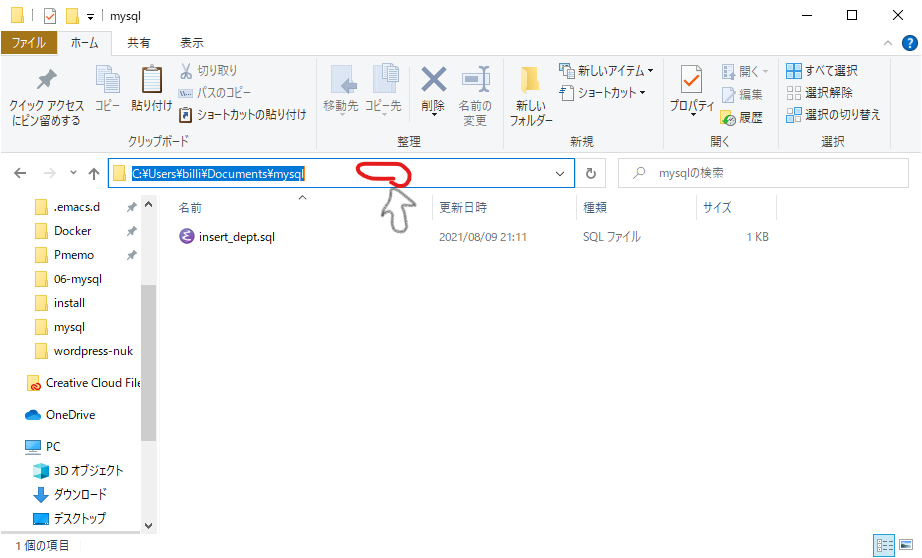
\includegraphics[width=10cm]{../06-mysql/03-cmd.png}
\vspace{3mm}

上の図のように、エクスプローラのアドレス欄の余白部分をクリックする。
すると、現在のフォルダをあらわす文字列が青く反転する。

\vspace{3mm}
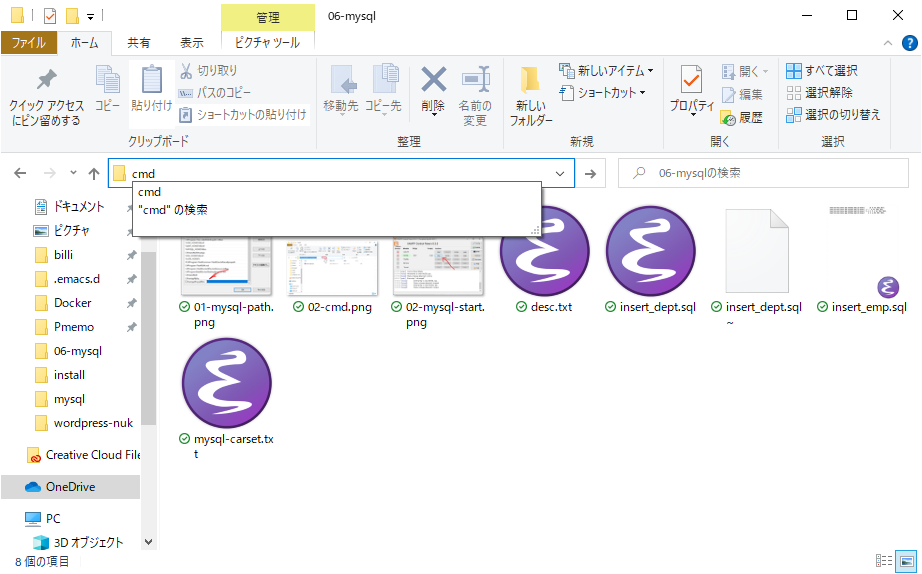
\includegraphics[width=10cm]{../06-mysql/04-cmd.png}
\vspace{3mm}

上の図のように、そこに ''\textsf{cmd}'' と入力して Enterキーを押下する。
すると、そのフォルダでコマンドプロンプトが起動する。

\vspace{3mm}
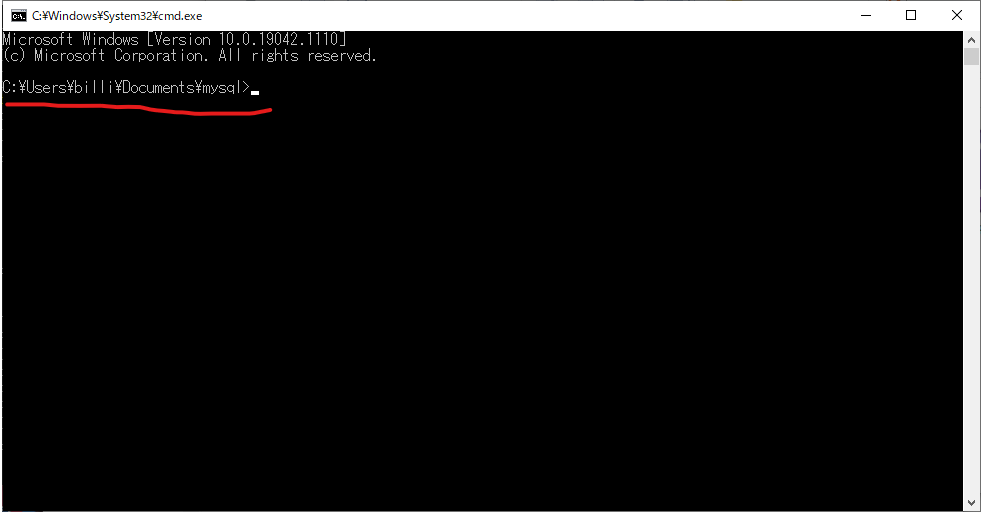
\includegraphics[width=11cm]{../06-mysql/05-cmd.png}
\vspace{3mm}

上の図の赤い線の部分が、現在のフォルダになっている。

\begin{tcolorbox}
 C:\yen Users\yen (ユーザー名)\yen Documents\yen mysql$>$ \textsf{dir}
\end{tcolorbox}

\textsf{dir} というコマンドを実行すると、現フォルダのファイルが一覧できる。
\textsf{insert\_dept.sql} があることがわかる。

\begin{verbatim}
 2021/08/09  22:05   <DIR>        .                (このフォルダ)
 2021/08/09  22:05   <DIR>        ..               (ひとつ上の階層)
 2021/08/09  22:05            222 dept.sql  
\end{verbatim}

\newpage

\subsubsection{ファイルを読み込んで、SQL文を実行する}

ここで、mysql を起動する。

\begin{tcolorbox}
 C:\yen Users\yen (ユーザー名)\yen Documents\yen mysql$>$ \textsf{mysql -u sampleuser -p} \\
 \textsf{Enter password: **********}
\end{tcolorbox}

\textsf{sample}データベースの使用を宣言する。

\begin{tcolorbox}
 MariaDB [(none)]$>$ \textsf{use sample;} \\
 MariaDB [sample]$>$
\end{tcolorbox}

次に、以下のコマンドで \textsf{insert\_dept.sql} を実行できる。

\begin{tcolorbox}
 MariaDB [sample]$>$ \textsf{source insert\_dept.sql}
\end{tcolorbox}

あるいは、以下のような省略形もある。

\begin{tcolorbox}
 MariaDB [sample]$>$ \textsf{\yen . insert\_dept.sql}
\end{tcolorbox}

確認する。

\begin{tcolorbox}
 MariaDB [sample]$>$ \textsf{select * from dept;}
\end{tcolorbox}

\begin{verbatim}
+-----+--------+
| id  | name   |
+-----+--------+
| 001 | 総務部 |
| 002 | 営業部 |
| 003 | 経理部 |
| 004 | 開発部 |
+-----+--------+
\end{verbatim}

読み込めているのがわかる。


\subsection{テーブル作成からデータの登録までを自動化する}

このことを応用して、テーブルの作成からデータの登録までを、ファイル読込みによって
自動化することができる。

以下のような記述が考えられる。

\begin{lstlisting}[caption=init\_data.sql]
 -- emp テーブルの作成
 -- もし empテーブルが存在しなかったら作成する。
 -- もし存在したら、このSQL文は実行されない。
 
 CREATE TABLE IF NOT EXISTS emp (
   id INT PRIMARY KEY AUTO_INCREMENT,
   name VARCHAR(20) NOT NULL,
   age INT NOT NULL,
   birthday YEAR NOT NULL,
   dept_id CHAR(3)
 );

 -- dept テーブルの作成
 -- もし deptテーブルが存在しなかったら作成する。
 -- もし存在したら、このSQL文は実行されない。
 
 CREATE TABLE IF NOT EXISTS dept (
   id CHAR(3) PRIMARY KEY,
   name VARCHAR(20) NOT NULL
 );

 -- もし、データが存在していたら、削除する。
 DELETE FROM emp;

 -- 自動連番を初期化する。
 ALTER TABLE emp AUTO_INCREMENT = 1;
 
 INSERT INTO emp (name, age, birthday, dept_id) VALUES
 ('菅原文太', 40, 1933, '001'),
 ('千葉真一', 34, 1939, '002') ,
 ('北大路欣也', 30, 1943, '003'),
 ('梶芽衣子', 26, 1947, '002');

 DELETE FROM dept;
 
 INSERT INTO dept (id, name) VALUES
 ('001', '総務部'),
 ('002', '営業部'),
 ('003', '経理部'),
 ('004', '開発部');

 SELECT * FROM emp;
 SELECT * FROM dept;
\end{lstlisting}

これを実行する。

\begin{tcolorbox}
 MariaDB [sample]$>$ \yen . init\_data.sql
\end{tcolorbox}

これにより、いつでもデータを初期状態に戻すことができるようになった。


\end{document}

%% 修正時刻: Sat May  2 15:10:04 2020


%% 修正時刻: Tue Aug 10 08:07:44 2021
